\documentclass[ngerman]{scrreprt}

\usepackage[utf8]{inputenc}
\usepackage[T1]{fontenc}
\usepackage{babel}
\usepackage{microtype}

\usepackage{blindtext}
\usepackage{graphicx} % JPG, PNG und PDF

\newcommand{\uzi}{Uwe Andreas Ziegenhagen}

\newcommand{\fk}[1]{\textbf{\textit{#1}}}


\title{Hallo Froscon!}
\author{Uwe Ziegenhagen}

\usepackage{hyperref}
\hypersetup{
    bookmarks=true,                     % show bookmarks bar
    unicode=false,                      % non - Latin characters in Acrobat’s bookmarks
    pdftoolbar=true,                        % show Acrobat’s toolbar
    pdfmenubar=true,                        % show Acrobat’s menu
    pdffitwindow=false,                 % window fit to page when opened
    pdfstartview={FitH},                    % fits the width of the page to the window
    pdftitle={My title},                        % title
    pdfauthor={Author},                 % author
    pdfsubject={Subject},                   % subject of the document
    pdfcreator={Creator},                   % creator of the document
    pdfproducer={Producer},             % producer of the document
    pdfkeywords={keyword1, key2, key3},   % list of keywords
    pdfnewwindow=true,                  % links in new window
    colorlinks=true,                        % false: boxed links; true: colored links
    linkcolor=blue,                          % color of internal links
    filecolor=blue,                     % color of file links
    citecolor=blue,                     % color of file links
    urlcolor=blue                        % color of external links
}



\begin{document}

\maketitle

\tableofcontents

\chapter{Froscon-Einführung}

\section{Einführung}

\subsection{Sankt Augustin}

\subsubsection{Nabel der Welt}


\blindtext[1]

\begin{itemize}
	\item Hallo
	\item Froscon
	\item Ich 
	\item bin 
	\item eine 
	\item Aufzählung
\end{itemize}

\begin{enumerate}
	\item Hallo
	\item Froscon
	
\begin{enumerate}
	\item Hallo
	\item Froscon
	\item Ich 
	\item bin 
	\item eine 
	\item Aufzählung
\end{enumerate}	
	
	\item Ich 
	\item bin 
	\item eine 
	\item Aufzählung
\end{enumerate}


\begin{description}
\item[Rot] \blindtext
\item[Grün] ist eine Farbe
\item[Blau] ist eine Farbe
\end{description}

\uzi

Hallo, dies ist ein \textbf{fettgedrucktes} Wort.

Hallo, dies ist ein \textit{kursives} Wort.

Hallo, dies ist ein \textbf{\textit{kursives}} Wort.

Hallo, ich \% bin ein \fk{Wort}

Siehe Abbildung \ref{fig:leopard} auf Seite \pageref{fig:leopard}.

\begin{figure}[htb]
\begin{center}
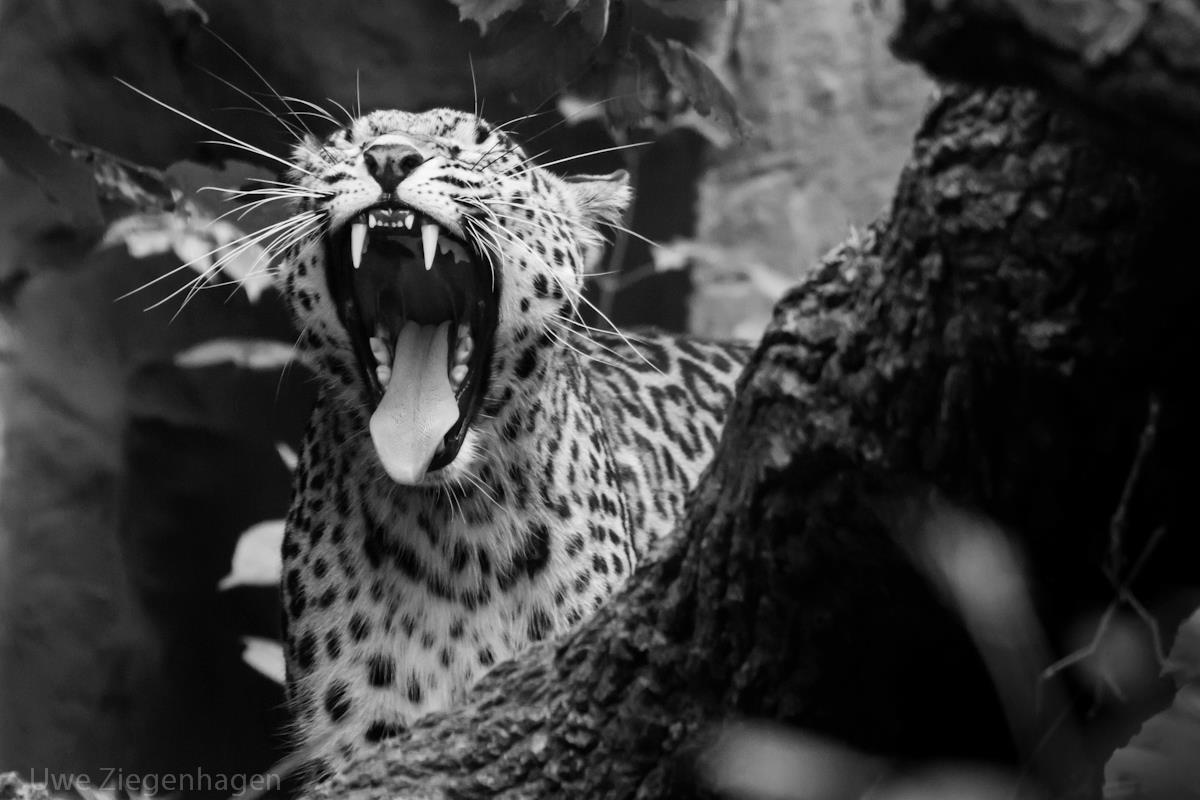
\includegraphics[width=\textwidth]{hallowelt}
\caption{Ich bin ein Leopard}\label{fig:leopard}
\end{center}
\end{figure}



\end{document}